\documentclass[12pt]{article}
\usepackage[margin=2.5cm]{geometry}
\usepackage{enumerate}
\usepackage{amsfonts}
\usepackage{amsmath}
\usepackage{fancyhdr}
\usepackage{amsmath}
\usepackage{amssymb}
\usepackage{amsthm}
\usepackage{mdframed}
\usepackage{graphicx}
\usepackage{subcaption}
\usepackage{adjustbox}
\usepackage{listings}
\usepackage{xcolor}
\usepackage{booktabs}
\usepackage[utf]{kotex}
\usepackage{hyperref}

\definecolor{codegreen}{rgb}{0,0.6,0}
\definecolor{codegray}{rgb}{0.5,0.5,0.5}
\definecolor{codepurple}{rgb}{0.58,0,0.82}
\definecolor{backcolour}{rgb}{0.95,0.95,0.92}

\lstdefinestyle{mystyle}{
    backgroundcolor=\color{backcolour},
    commentstyle=\color{codegreen},
    keywordstyle=\color{magenta},
    numberstyle=\tiny\color{codegray},
    stringstyle=\color{codepurple},
    basicstyle=\ttfamily\footnotesize,
    breakatwhitespace=false,
    breaklines=true,
    captionpos=b,
    keepspaces=true,
    numbers=left,
    numbersep=5pt,
    showspaces=false,
    showstringspaces=false,
    showtabs=false,
    tabsize=1
}

\lstset{style=mystyle}

\pagestyle{fancy}
\renewcommand{\headrulewidth}{0.4pt}
\lhead{Team Treehouse}
\rhead{Java Objects Part 4 Notes}

\begin{document}
\title{Java Objects Part 4 Notes}
\author{Team Treehouse}
\maketitle

\section{Exceptions}

\bigskip

\begin{center}
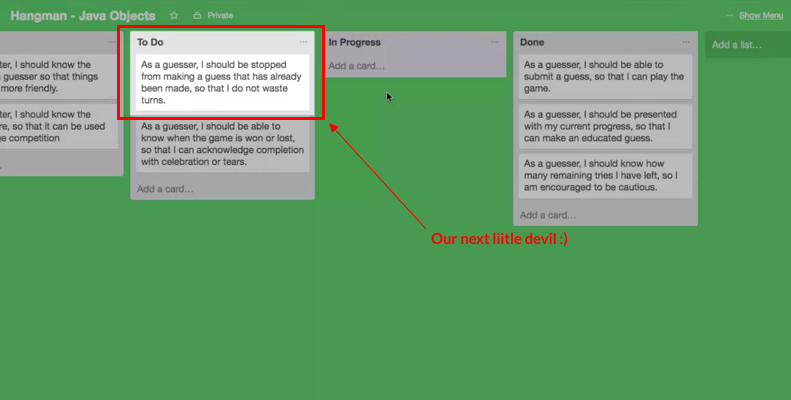
\includegraphics[width=\linewidth]{images/part_4_notes_1.png}
\end{center}

\begin{itemize}
    \item \textit{throw new EXCEPTION\_NAME:} raises exception \textit{EXCPETION\_NAME}
    \item \textit{try} and \textit{catch:} handles expections

    \begin{lstlisting}[language=Java,caption={lesson\_01/Game.java}]
    public class Game {
        ...
        public boolean applyGuess(char letter) {
            if (misses.indexOf(letter) != -1 || hits.indexOf(letter) != -1) {
                throw new IllegalArgumentException(letter + " has already been guessed"); // <- this little guy here :)
            }

            ...
        }

        ...
    }
    \end{lstlisting}

    \begin{lstlisting}[language=Java,caption={lesson\_01/Prompter.java}]
    import java.util.Scanner;

    public class Prompter {
        ...
        public boolean promptForGuess() {
            ...
            boolean isHit = false;
            try { // <- And this little guy here :)
                isHit = game.applyGuess(guess);
            } catch (IllegalArgumentException iae) {
                System.out.println(iae.getMessage());
            }

            return isHit;
        }
    }
    \end{lstlisting}

    \bigskip

    \underline{\textbf{Notes:}}

    \bigskip

    \begin{itemize}
        \item Files can be compiled and displayed by typing \textit{javac Hangman.java \&\& java Hangman}
        in terminal
    \end{itemize}
\end{itemize}

\bigskip

\section{Validating and Normalizing User Input}

\bigskip


\begin{center}
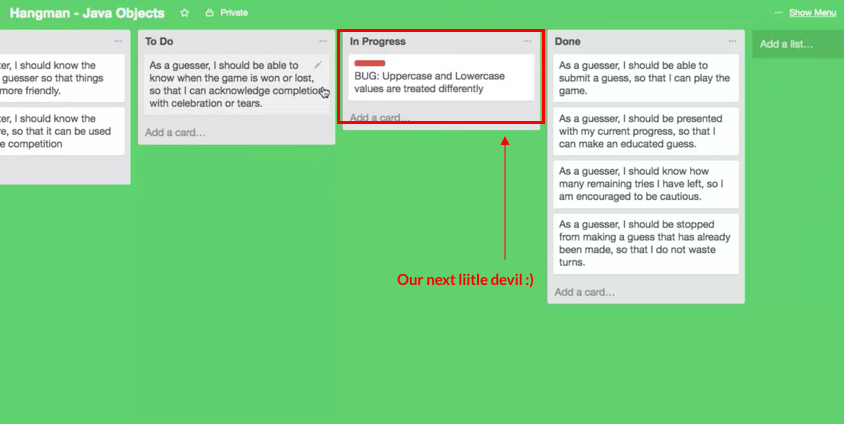
\includegraphics[width=\linewidth]{images/part_4_notes_2.png}
\end{center}

\begin{itemize}
    \item \textit{Character.toLowercase(CHAR\_VAR)}: turns value in \textit{CHAR\_VAR}
    to a lowercase character


    \begin{lstlisting}[language=Java,caption={lesson\_02/Game.java}]
    public class Game {
        ...
        private char normalizeGuess(char letter) {
            ...
            letter = Character.toLowercase(letter); // <- This little guy here :)
            ...
        }
    }
    \end{lstlisting}

    \bigskip

    \underline{\textbf{Notes:}}

    \bigskip

    \begin{itemize}
        \item Files can be compiled and displayed by typing \textit{javac Hangman.java \&\& java Hangman}
        in terminal
    \end{itemize}
\end{itemize}

\bigskip

\section{Exercise 1}

\bigskip

\begin{itemize}
    \item Solution included in \textit{exercise\_1.java}
\end{itemize}

\bigskip

\section{Using Method Overloading}

\bigskip

\begin{center}
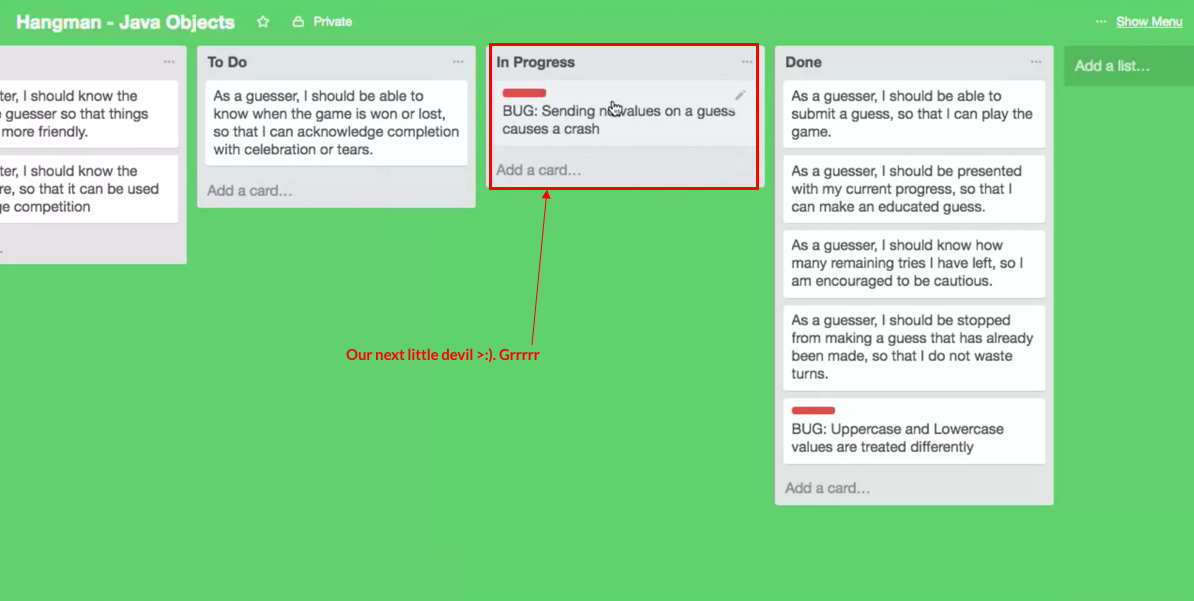
\includegraphics[width=\linewidth]{images/part_4_notes_3.png}
\end{center}

\bigskip

\underline{\textbf{Notes:}}

\bigskip

\begin{itemize}
    \item Files can be compiled and displayed by typing \textit{javac Hangman.java \&\& java Hangman}
    in terminal
\end{itemize}

\bigskip

\section{Determining if the Game is Won}

\bigskip

\begin{center}
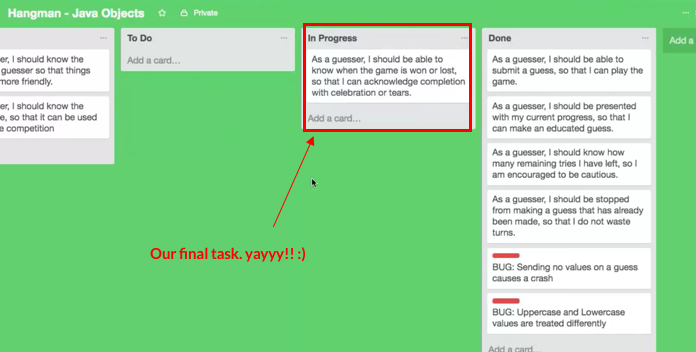
\includegraphics[width=\linewidth]{images/part_4_notes_5.png}
\end{center}

\bigskip

\underline{\textbf{Notes:}}

\bigskip

\begin{itemize}
    \item Files can be compiled and displayed by typing \textit{javac Hangman.java \&\& java Hangman}
    in terminal
\end{itemize}

\bigskip

\section{Quiz 1}

\bigskip

\begin{enumerate}[1.]
    \item

    Below is some code for a carnival based Dunk Tank. As long as there are tries
    remaining and the person has not been dunked keep throwing the ball.

    Please choose the answer that properly fills in the blanks with the proper code
    for the while loop

    \bigskip

    \begin{lstlisting}[language=Java,caption={lesson\_02/Game.java}]
    int remainingTries = 3;
    while (remainingTries __ 0 __ __ dunkTank.isDunked()) {
        throwBall();
    }
    \end{lstlisting}

    \begin{enumerate}[A.]
        \item \textgreater,\&\&,!
        \item =,||,!
        \item !=,||,@
    \end{enumerate}

    \bigskip

    \textbf{Answer:} A

    \item

    Due to the separation we have chosen, what outcome can we expect?

    \bigskip

    \begin{enumerate}[A.]
        \item We will be able to run this in other languages like JavaScript or Python.
        \item We can more easily generate code using external tools.
        \item We will be able to use the same game logic in other applications, such as console applications, web sites and apps.
    \end{enumerate}

    \bigskip

    \textbf{Answer:} C

\end{enumerate}

\bigskip

\section{Arrays and Command Line Arguments}

\bigskip

\begin{itemize}
    \item \textit{string[] args:} represent arguments passed in commandline


    \begin{lstlisting}[language=Bash]
    >>> java Hangman corgi # <- 'corgi' is stored in args[0]
    \end{lstlisting}

    \bigskip

    \underline{\textbf{Example:}}


    \begin{lstlisting}[language=Java,caption={lesson\_07/Hangman.java}]
    public class Hangman {

        public static void main(String[] args) { // <- this guy here :)

            if (args.length == 0) {
                System.out.println("Usage: java Hangman <answer>");
                System.err.println("Answer is required");
                System.exit(1);
            }
            Game game = new Game(args[0]);
            ...
        }

    }
    \end{lstlisting}

    \underline{\textbf{Notes:}}

    \bigskip

    \begin{itemize}
        \item Files can be compiled and displayed by typing \textit{javac Hangman.java \&\& java Hangman \textless answer \textgreater}
        in terminal
        \begin{itemize}
            \item i.e. javac Hangman.java \&\& java Hangman corgi
        \end{itemize}
    \end{itemize}
\end{itemize}

\bigskip

\section{Wrapping Up}

\bigskip

\section{Exercise 2}

\bigskip

\begin{itemize}
    \item Solution included in \textit{exercise\_2.java}
\end{itemize}

\bigskip

\section{Quiz 2}

\bigskip

\begin{enumerate}[1.]
    \item

    String[] fruits = \{"apple", "banana", "cherry"\};

    How do you tell how many items are in the fruits array?

    \bigskip

    \begin{enumerate}[A.]
        \item fruits.length;
        \item len(fruits);
        \item fruits.count();
        \item fruits.size();
    \end{enumerate}

    \bigskip

    \textbf{Answer:} A

    \item

    How would you select the first element of this array: String[] fruits =
    \{"apple", "banana", "cherry"\};

    \bigskip

    \begin{enumerate}[A.]
        \item fruits[0];
        \item fruits[1];
        \item fruits.first;
    \end{enumerate}

    \bigskip

    \textbf{Answer:} A

    \item Strings can be thought of as an array of characters.

    \bigskip

    \begin{enumerate}[A.]
        \item True
        \item False
    \end{enumerate}

    \bigskip

    \textbf{Answer:} A

    \item Assuming there is a compiled java class named HelloWorld with a static
    method named main that accepts an Array of Strings named args...

    \bigskip

    What would be stored in args[1] if we ran java HelloWorld Luke Skywalker

    \bigskip

    \begin{enumerate}[A.]
        \item Darth
        \item Luke Skywalker
        \item Skywalker
        \item Luke
    \end{enumerate}

    \bigskip

    \textbf{Answer:} C

\end{enumerate}


\end{document}